\subsection{Covariance initialization improves two-call KID and coverage}
\label{sec:cifar}
Covariance initialization lowers two-call KID by 32.0\% and raises
real-data coverage from 0.206 to 0.288 (Fig.~\ref{fig:cifar_initializer}).
KID falls from 0.1858 to 0.1264, a paired difference of
$-0.05938$ [$-0.06138,-0.05739$] with nominal 95\% simultaneous coverage across five prespecified
Student-$t$ contrasts under the panel-effect approximation. Full-moment initialization has
similar coverage (0.290) and higher KID (0.1405). DPM++ and UniPC coincide
in this two-call comparison at KID 0.2225.
KID compares distributions in Inception feature space~\cite{binkowski2018demystifying}.
DINO coverage is the fraction of real reference neighborhoods reached
by generated features~\cite{naeem2020density}.

The experiment uses a public pretrained CIFAR-10 DDPM
\cite{krizhevsky2009cifar,ho2020ddpm}. A 20,000-image DDIM100 teacher supplies
5,000/5,000/10,000 disjoint fitting/calibration/evaluation images.
The original 22-arm study used a 2,048-image pilot and 10,000 fresh images
per arm. An ablation on its paired seeds yielded KID of 0.2054 for mean
only, 0.1413 for full moments, and 0.1261 for covariance only. It motivated
the separate six-arm confirmation on five fresh paired panels of 2,000
images from the same checkpoint. Uncertainty is over generated panels and
conditions on the fixed real-data reference (Supp.~Sec.~F.3).

The repair improves agreement with real data while leaving a large
teacher-relative deficit. Nine of ten teacher-defined DINO regions
remain depleted, and conditional spread remains contracted. The largest region holds 35.35\% of teacher images, 97.30\%
of standard two-call outputs, and 91.29\% after the covariance start
(Supp.~Sec.~C.6). The fraction within the real-training 1--99\% frequency
range rises from 0.72\% to 24.7\%, compared with 97.2\% for DDIM200
(Supp.~Secs.~F.6 and G.1).

\begin{figure}[t]
\centering
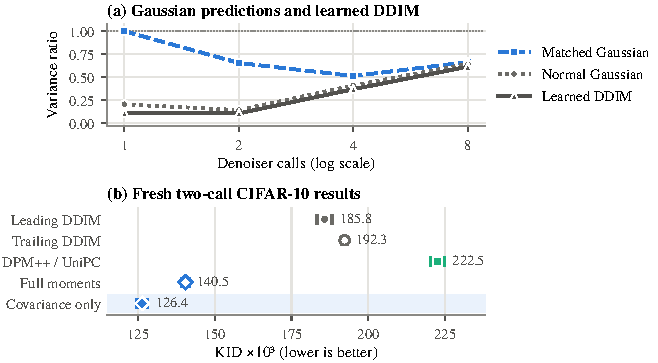
\includegraphics[width=\linewidth]{../figures/initialization_repair.pdf}
\caption{Correcting the initial covariance improves two-call generation.
(a) Saved Gaussian predictions and learned observations use a common
teacher-fit pixel basis and distinguish initialization from integration.
(b) Fresh confirmation with ordinary 95\% Student-$t$ intervals over five
generated-sample panels. DPM++ and UniPC coincide in this comparison.}
\label{fig:cifar_initializer}
\end{figure}

To explain why the starting covariance matters, consider a centered clean
Gaussian coordinate $X_0$ with variance
$\lambda>0$. Variance-preserving noising gives
$X_t=\sqrt{\bar\alpha_t}X_0+\sqrt{1-\bar\alpha_t}\,\epsilon$ at
timestep $t$, with cumulative signal coefficient $\bar\alpha_t\in[0,1]$
and independent $\epsilon\sim\mathcal N(0,1)$. Write
$v_t=\bar\alpha_t\lambda+1-\bar\alpha_t$ for the noisy variance and
$u_t=(\sqrt{\bar\alpha_t\lambda},\sqrt{1-\bar\alpha_t})$.
With the conditional mean noise predictor $\mathbb E[\epsilon\mid X_t]$
and no clipping, a deterministic DDIM
transition to an earlier timestep $s$ multiplies the coordinate by
$\sqrt{v_s/v_t}\cos\angle(u_s,u_t)$. The variance factors telescope on a
fixed grid to the clean endpoint:
\begin{equation}
\frac{\operatorname{Var}(X_{\rm out})}{\lambda}
=\underbrace{\frac{\nu_{\rm start}}{v_{\rm start}}}_{\text{initialization}}
\underbrace{\prod_{t\rightarrow s}\cos^2\angle(u_s,u_t)}_{\text{integration}},
\label{eq:gaussian}
\end{equation}
where $X_{\rm out}$ is the final coordinate, $\nu_{\rm start}$ and
$v_{\rm start}$ are actual and matched starting variances, and the product
runs over adjacent grid transitions~\cite{benita2025spectral,pierret2025gaussian}.
Matching the noisy marginal sets the first factor to one. Refining the same
endpoints improves the second factor by $\cos b\cos c\geq\cos(b+c)$
for nonnegative angles $b,c$ with $b+c\leq\pi/2$. Changing the leading-grid
budget also changes the starting timestep. The saved Gaussian predictions
give standard-normal to matched aggregate variance ratios 0.216, 0.800,
and 0.968 at two, four, and eight calls.

For a leading grid starting at timestep $t_0$, the tested initializer is
\begin{equation}
X_{\rm start}=
\big[(1-\bar\alpha_{t_0})I+\bar\alpha_{t_0}\widehat C\big]^{1/2}Z,
\qquad Z\sim\mathcal N(0,I),
\label{eq:covariance_start}
\end{equation}
where $X_{\rm start}$ is the initial noisy image, $Z$ is standard Gaussian
noise, and $I$ is the identity in 3,072-dimensional pixel space. The clean
covariance estimate $\widehat C$ uses 128 teacher-fit pixel components
and an isotropic residual. The square root is symmetric.
The two-call grid starts at $t_0=500$. The initializer changes the start
with no additional denoiser calls. Equation~\ref{eq:gaussian} extends
directionwise to shared eigenvectors. Learned trajectories at four/eight
calls correlate with the Gaussian prediction (Spearman 0.938/0.894), but
also exhibit mixing. The exact Gaussian derivation and the learned-model
checks are in Supp.~Secs.~D--F.


Evaluating the unchanged generated outputs against CIFAR-10.1v6
\cite{recht2018cifar10} lowers KID from 0.19060 to 0.12832
(32.7\%) and raises coverage from 0.3221 to 0.4268, with precision
falling from 0.9756 to 0.9580.
The paired KID difference is $-0.06228$ [$-0.06422,-0.06035$],
with 95\% simultaneous coverage across four contrasts (Supp.~Sec.~F.4).
All four prespecified KID contrasts retain their direction against this
reference, including the adverse output-map comparison below. The intervals
condition on the fixed 2,000 reference images.

\subsection{Intervention location separates spread from useful coverage}
\label{sec:numerical}
At four calls, output covariance restoration raises
pixel variance ratio from 0.376 to 0.917, while coverage falls from 0.478 to
0.332 and KID worsens from 0.0903 to 0.1024
(Fig.~\ref{fig:numerical_repair}). UniPC instead reaches coverage 0.549 and
KID 0.0694. At eight calls, output restoration again worsens KID
(0.0363 to 0.0505), while UniPC reaches 0.0245 (Supp.~Table~6).
These original frozen
comparisons retain the practical prediction transforms and clipping;
matched-grid controls hold trailing timesteps fixed, for which four-call
DDIM has KID 0.1132. Covariance-aware sampling~\cite{schioppa2026covariance}
does not improve this checkpoint within the four/eight-call ceilings when
forward and Jacobian--vector-product calls are both counted. The supplement
retains those controls and each declared cost convention.

\begin{figure}[t]
\centering
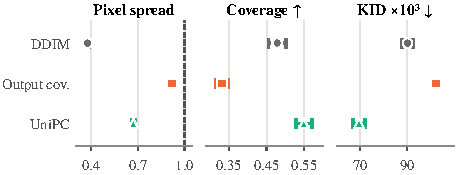
\includegraphics[width=\linewidth]{../figures/numerical_repair.pdf}
\caption{Restoring output spread can degrade useful coverage.
Four-call CIFAR-10 interventions: five paired 2,000-image panels, ordinary
95\% Student-$t$ intervals. Pixel spread is teacher-relative; coverage and KID use real data.}
\label{fig:numerical_repair}
\end{figure}

An independently pretrained variance-preserving EDM model~\cite{karras2022edm}
gives a matched-call solver comparison (Fig.~\ref{fig:edm_solver_audit}).
At 15 calls, Heun lowers KID from 0.00876 to 0.00250 while coverage falls
from 0.477 to 0.417. At 35 calls, it lowers KID from 0.00250 to 0.000413
with coverage 0.501 for both solvers. At three and seven calls, its fewer,
larger steps give worse KID. Heun uses $2K-1$ calls for $K$ integration
steps. At seven calls, Heun achieves DINO precision of 0.906, while
24.7\% of its images fall within the real-training frequency range.
This mismatch shows the value of the complementary frequency check
(Supp.~Sec.~G.1).

\begin{figure}[t]
\centering
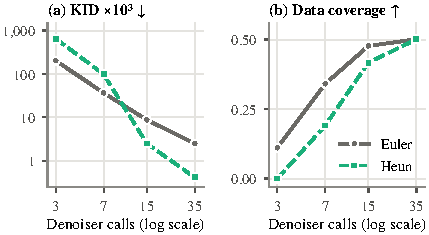
\includegraphics[width=\linewidth]{../figures/edm_solver_audit.pdf}
\caption{EDM solver choice changes with budget.
All eight arms share 2,048 noise inputs; calls and integration steps differ.
KID uses a logarithmic scale. Points are descriptive, without model-seed
uncertainty; lines connect the evaluated budgets.}
\label{fig:edm_solver_audit}
\end{figure}
